\documentclass[twoside]{book}

% Packages required by doxygen
\usepackage{fixltx2e}
\usepackage{calc}
\usepackage{doxygen}
\usepackage[export]{adjustbox} % also loads graphicx
\usepackage{graphicx}
\usepackage[utf8]{inputenc}
\usepackage{makeidx}
\usepackage{multicol}
\usepackage{multirow}
\PassOptionsToPackage{warn}{textcomp}
\usepackage{textcomp}
\usepackage[nointegrals]{wasysym}
\usepackage[table]{xcolor}

% Font selection
\usepackage[T1]{fontenc}
\usepackage[scaled=.90]{helvet}
\usepackage{courier}
\usepackage{amssymb}
\usepackage{sectsty}
\renewcommand{\familydefault}{\sfdefault}
\allsectionsfont{%
  \fontseries{bc}\selectfont%
  \color{darkgray}%
}
\renewcommand{\DoxyLabelFont}{%
  \fontseries{bc}\selectfont%
  \color{darkgray}%
}
\newcommand{\+}{\discretionary{\mbox{\scriptsize$\hookleftarrow$}}{}{}}

% Page & text layout
\usepackage{geometry}
\geometry{%
  a4paper,%
  top=2.5cm,%
  bottom=2.5cm,%
  left=2.5cm,%
  right=2.5cm%
}
\tolerance=750
\hfuzz=15pt
\hbadness=750
\setlength{\emergencystretch}{15pt}
\setlength{\parindent}{0cm}
\setlength{\parskip}{3ex plus 2ex minus 2ex}
\makeatletter
\renewcommand{\paragraph}{%
  \@startsection{paragraph}{4}{0ex}{-1.0ex}{1.0ex}{%
    \normalfont\normalsize\bfseries\SS@parafont%
  }%
}
\renewcommand{\subparagraph}{%
  \@startsection{subparagraph}{5}{0ex}{-1.0ex}{1.0ex}{%
    \normalfont\normalsize\bfseries\SS@subparafont%
  }%
}
\makeatother

% Headers & footers
\usepackage{fancyhdr}
\pagestyle{fancyplain}
\fancyhead[LE]{\fancyplain{}{\bfseries\thepage}}
\fancyhead[CE]{\fancyplain{}{}}
\fancyhead[RE]{\fancyplain{}{\bfseries\leftmark}}
\fancyhead[LO]{\fancyplain{}{\bfseries\rightmark}}
\fancyhead[CO]{\fancyplain{}{}}
\fancyhead[RO]{\fancyplain{}{\bfseries\thepage}}
\fancyfoot[LE]{\fancyplain{}{}}
\fancyfoot[CE]{\fancyplain{}{}}
\fancyfoot[RE]{\fancyplain{}{\bfseries\scriptsize Generated by Doxygen }}
\fancyfoot[LO]{\fancyplain{}{\bfseries\scriptsize Generated by Doxygen }}
\fancyfoot[CO]{\fancyplain{}{}}
\fancyfoot[RO]{\fancyplain{}{}}
\renewcommand{\footrulewidth}{0.4pt}
\renewcommand{\chaptermark}[1]{%
  \markboth{#1}{}%
}
\renewcommand{\sectionmark}[1]{%
  \markright{\thesection\ #1}%
}

% Indices & bibliography
\usepackage{natbib}
\usepackage[titles]{tocloft}
\setcounter{tocdepth}{3}
\setcounter{secnumdepth}{5}
\makeindex

% Hyperlinks (required, but should be loaded last)
\usepackage{ifpdf}
\ifpdf
  \usepackage[pdftex,pagebackref=true]{hyperref}
\else
  \usepackage[ps2pdf,pagebackref=true]{hyperref}
\fi
\hypersetup{%
  colorlinks=true,%
  linkcolor=blue,%
  citecolor=blue,%
  unicode%
}

% Custom commands
\newcommand{\clearemptydoublepage}{%
  \newpage{\pagestyle{empty}\cleardoublepage}%
}

\usepackage{caption}
\captionsetup{labelsep=space,justification=centering,font={bf},singlelinecheck=off,skip=4pt,position=top}

%===== C O N T E N T S =====

\begin{document}

% Titlepage & ToC
\hypersetup{pageanchor=false,
             bookmarksnumbered=true,
             pdfencoding=unicode
            }
\pagenumbering{roman}
\begin{titlepage}
\vspace*{7cm}
\begin{center}%
{\Large Lane Detection Module \\[1ex]\large 1.\+0 }\\
\vspace*{1cm}
{\large Generated by Doxygen 1.8.11}\\
\end{center}
\end{titlepage}
\clearemptydoublepage
\tableofcontents
\clearemptydoublepage
\pagenumbering{arabic}
\hypersetup{pageanchor=true}

%--- Begin generated contents ---
\chapter{Class Index}
\section{Class List}
Here are the classes, structs, unions and interfaces with brief descriptions\+:\begin{DoxyCompactList}
\item\contentsline{section}{\hyperlink{classFrameParser}{Frame\+Parser} \\*Class \hyperlink{classFrameParser}{Frame\+Parser} The following class \hyperlink{classFrameParser}{Frame\+Parser} aids \hyperlink{classUserInterface}{User\+Interface} class by parsing the frames in a video and calling the \hyperlink{classVisionModule}{Vision\+Module} and \hyperlink{classUserInterface}{User\+Interface} class for further image processing using Open\+CV }{\pageref{classFrameParser}}{}
\item\contentsline{section}{\hyperlink{classUserInterface}{User\+Interface} \\*Class \hyperlink{classUserInterface}{User\+Interface} The following class \hyperlink{classUserInterface}{User\+Interface} gets the user input and interacts with the \hyperlink{classVisionModule}{Vision\+Module} class. It augments the output from \hyperlink{classVisionModule}{Vision\+Module} class onto the user input }{\pageref{classUserInterface}}{}
\item\contentsline{section}{\hyperlink{classVisionModule}{Vision\+Module} \\*Class \hyperlink{classVisionModule}{Vision\+Module} The following class \hyperlink{classVisionModule}{Vision\+Module} gets the frames from \hyperlink{classFrameParser}{Frame\+Parser} class and is responsible for filtering and detecting hough lines on to an image }{\pageref{classVisionModule}}{}
\end{DoxyCompactList}

\chapter{File Index}
\section{File List}
Here is a list of all documented files with brief descriptions\+:\begin{DoxyCompactList}
\item\contentsline{section}{app/\hyperlink{FrameParser_8cpp}{Frame\+Parser.\+cpp} \\*Implements \hyperlink{classFrameParser}{Frame\+Parser} class methods }{\pageref{FrameParser_8cpp}}{}
\item\contentsline{section}{app/\hyperlink{VisionModule_8cpp}{Vision\+Module.\+cpp} \\*Implements \hyperlink{classVisionModule}{Vision\+Module} class methods }{\pageref{VisionModule_8cpp}}{}
\item\contentsline{section}{include/\hyperlink{FrameParser_8h}{Frame\+Parser.\+h} \\*\hyperlink{classFrameParser}{Frame\+Parser} Class declaration  Declared functions Class to extract frames from the video input, and process frames }{\pageref{FrameParser_8h}}{}
\item\contentsline{section}{include/\hyperlink{UserInterface_8h}{User\+Interface.\+h} \\*\hyperlink{classUserInterface}{User\+Interface} Class declaration  Declared function Class to interact with user about the input format and to display the lanes and text on top of the video }{\pageref{UserInterface_8h}}{}
\item\contentsline{section}{include/\hyperlink{VisionModule_8h}{Vision\+Module.\+h} \\*\hyperlink{classVisionModule}{Vision\+Module} Class declaration  Declared functions Class to denoise frames, apply homography, apply histogram, and find heading angle }{\pageref{VisionModule_8h}}{}
\item\contentsline{section}{test/\hyperlink{FrameParserTest_8cpp}{Frame\+Parser\+Test.\+cpp} \\*Implements tests for \hyperlink{classFrameParser}{Frame\+Parser} class methods }{\pageref{FrameParserTest_8cpp}}{}
\item\contentsline{section}{test/\hyperlink{UserInterfaceTest_8cpp}{User\+Interface\+Test.\+cpp} \\*Unit test for the \hyperlink{classUserInterface}{User\+Interface} class }{\pageref{UserInterfaceTest_8cpp}}{}
\item\contentsline{section}{test/\hyperlink{VisionModuleTest_8cpp}{Vision\+Module\+Test.\+cpp} \\*Test for \hyperlink{classVisionModule}{Vision\+Module} class methods }{\pageref{VisionModuleTest_8cpp}}{}
\end{DoxyCompactList}

\chapter{Class Documentation}
\hypertarget{classFrameParser}{}\section{Frame\+Parser Class Reference}
\label{classFrameParser}\index{Frame\+Parser@{Frame\+Parser}}


Class \hyperlink{classFrameParser}{Frame\+Parser} The following class \hyperlink{classFrameParser}{Frame\+Parser} aids \hyperlink{classUserInterface}{User\+Interface} class by parsing the frames in a video and calling the \hyperlink{classVisionModule}{Vision\+Module} and \hyperlink{classUserInterface}{User\+Interface} class for further image processing using Open\+CV.  




{\ttfamily \#include $<$Frame\+Parser.\+h$>$}

\subsection*{Public Member Functions}
\begin{DoxyCompactItemize}
\item 
\hyperlink{classFrameParser_adf34f5de47578ffa08286152d50ce43f}{Frame\+Parser} ()
\begin{DoxyCompactList}\small\item\em constructor \hyperlink{classFrameParser}{Frame\+Parser} \end{DoxyCompactList}\item 
\hyperlink{classFrameParser_a844ec6e5e1978dbf60944a072f4bbadc}{$\sim$\+Frame\+Parser} ()
\begin{DoxyCompactList}\small\item\em destructor \hyperlink{classFrameParser}{Frame\+Parser} \end{DoxyCompactList}\item 
int \hyperlink{classFrameParser_aa3b62170c32136f78af7465bf13d4485}{extract\+Frame} (\hyperlink{classUserInterface}{User\+Interface} interface, bool test)
\begin{DoxyCompactList}\small\item\em Function extract\+Frames. \end{DoxyCompactList}\end{DoxyCompactItemize}


\subsection{Detailed Description}
Class \hyperlink{classFrameParser}{Frame\+Parser} The following class \hyperlink{classFrameParser}{Frame\+Parser} aids \hyperlink{classUserInterface}{User\+Interface} class by parsing the frames in a video and calling the \hyperlink{classVisionModule}{Vision\+Module} and \hyperlink{classUserInterface}{User\+Interface} class for further image processing using Open\+CV. 

\subsection{Constructor \& Destructor Documentation}
\index{Frame\+Parser@{Frame\+Parser}!Frame\+Parser@{Frame\+Parser}}
\index{Frame\+Parser@{Frame\+Parser}!Frame\+Parser@{Frame\+Parser}}
\subsubsection[{\texorpdfstring{Frame\+Parser()}{FrameParser()}}]{\setlength{\rightskip}{0pt plus 5cm}Frame\+Parser\+::\+Frame\+Parser (
\begin{DoxyParamCaption}
{}
\end{DoxyParamCaption}
)}\hypertarget{classFrameParser_adf34f5de47578ffa08286152d50ce43f}{}\label{classFrameParser_adf34f5de47578ffa08286152d50ce43f}


constructor \hyperlink{classFrameParser}{Frame\+Parser} 


\begin{DoxyParams}{Parameters}
{\em none} & \\
\hline
\end{DoxyParams}
\begin{DoxyReturn}{Returns}
none 
\end{DoxyReturn}
\index{Frame\+Parser@{Frame\+Parser}!````~Frame\+Parser@{$\sim$\+Frame\+Parser}}
\index{````~Frame\+Parser@{$\sim$\+Frame\+Parser}!Frame\+Parser@{Frame\+Parser}}
\subsubsection[{\texorpdfstring{$\sim$\+Frame\+Parser()}{~FrameParser()}}]{\setlength{\rightskip}{0pt plus 5cm}Frame\+Parser\+::$\sim$\+Frame\+Parser (
\begin{DoxyParamCaption}
{}
\end{DoxyParamCaption}
)}\hypertarget{classFrameParser_a844ec6e5e1978dbf60944a072f4bbadc}{}\label{classFrameParser_a844ec6e5e1978dbf60944a072f4bbadc}


destructor \hyperlink{classFrameParser}{Frame\+Parser} 


\begin{DoxyParams}{Parameters}
{\em none} & \\
\hline
\end{DoxyParams}
\begin{DoxyReturn}{Returns}
none 
\end{DoxyReturn}


\subsection{Member Function Documentation}
\index{Frame\+Parser@{Frame\+Parser}!extract\+Frame@{extract\+Frame}}
\index{extract\+Frame@{extract\+Frame}!Frame\+Parser@{Frame\+Parser}}
\subsubsection[{\texorpdfstring{extract\+Frame(\+User\+Interface interface, bool test)}{extractFrame(UserInterface interface, bool test)}}]{\setlength{\rightskip}{0pt plus 5cm}int Frame\+Parser\+::extract\+Frame (
\begin{DoxyParamCaption}
\item[{{\bf User\+Interface}}]{interface, }
\item[{bool}]{test}
\end{DoxyParamCaption}
)}\hypertarget{classFrameParser_aa3b62170c32136f78af7465bf13d4485}{}\label{classFrameParser_aa3b62170c32136f78af7465bf13d4485}


Function extract\+Frames. 


\begin{DoxyParams}{Parameters}
{\em interface} & of type \hyperlink{classUserInterface}{User\+Interface} \\
\hline
{\em test} & of type bool \\
\hline
\end{DoxyParams}
\begin{DoxyReturn}{Returns}
0 if the program is successful else -\/1 The following function will extract frames from the video input and using the frames calls \hyperlink{classVisionModule}{Vision\+Module} and user\+Interface class 
\end{DoxyReturn}


The documentation for this class was generated from the following files\+:\begin{DoxyCompactItemize}
\item 
include/\hyperlink{FrameParser_8h}{Frame\+Parser.\+h}\item 
app/\hyperlink{FrameParser_8cpp}{Frame\+Parser.\+cpp}\end{DoxyCompactItemize}

\hypertarget{classUserInterface}{}\section{User\+Interface Class Reference}
\label{classUserInterface}\index{User\+Interface@{User\+Interface}}


Class \hyperlink{classUserInterface}{User\+Interface} The following class \hyperlink{classUserInterface}{User\+Interface} gets the user input and interacts with the \hyperlink{classVisionModule}{Vision\+Module} class. It augments the output from \hyperlink{classVisionModule}{Vision\+Module} class onto the user input.  




{\ttfamily \#include $<$User\+Interface.\+h$>$}

\subsection*{Public Member Functions}
\begin{DoxyCompactItemize}
\item 
\hyperlink{classUserInterface_ae6fb70370701b3bd6120e923df9705b0}{User\+Interface} ()
\begin{DoxyCompactList}\small\item\em Default constructor \hyperlink{classUserInterface}{User\+Interface}. \end{DoxyCompactList}\item 
\hyperlink{classUserInterface_a0d6b9486d437a4d18c5a7bec6781de9a}{User\+Interface} (int, const std\+::string \&, int, const std\+::string \&)
\begin{DoxyCompactList}\small\item\em constructor \hyperlink{classUserInterface}{User\+Interface} \end{DoxyCompactList}\item 
\hyperlink{classUserInterface_ae588b2ff1711a016dd4c6fc5002c0841}{$\sim$\+User\+Interface} ()
\begin{DoxyCompactList}\small\item\em destructor \hyperlink{classUserInterface}{User\+Interface} \end{DoxyCompactList}\item 
std\+::string \hyperlink{classUserInterface_a90bc99e42cda74b901cad6983b8081c7}{return\+Default\+Choice} ()
\begin{DoxyCompactList}\small\item\em Function return\+Default\+Choice. \end{DoxyCompactList}\item 
void \hyperlink{classUserInterface_a4d4098f59d11a180704a5f8e415fa4fd}{get\+User\+Choice} ()
\begin{DoxyCompactList}\small\item\em Function get\+User\+Choice. \end{DoxyCompactList}\item 
int \hyperlink{classUserInterface_a65eb4d8676fe792af4dd037084273421}{return\+User\+Choice} ()
\begin{DoxyCompactList}\small\item\em Function return\+User\+Choice. \end{DoxyCompactList}\item 
void \hyperlink{classUserInterface_acb2302084e8e62740a6e6720bbb700ea}{get\+Input\+Location} ()
\begin{DoxyCompactList}\small\item\em Function get\+Input\+Location. \end{DoxyCompactList}\item 
std\+::string \hyperlink{classUserInterface_aaf13bdcbe482d0f316f2c50865d52220}{return\+Input\+Location} ()
\begin{DoxyCompactList}\small\item\em Function return\+Input\+Location. \end{DoxyCompactList}\item 
int \hyperlink{classUserInterface_af5b3c6e8b1719219aca2cf17e90304ec}{return\+Camera\+ID} ()
\begin{DoxyCompactList}\small\item\em Function return\+Camera\+ID. \end{DoxyCompactList}\item 
void \hyperlink{classUserInterface_af86d444796c9627349419868b460c5c7}{display\+Lanes} (cv\+::\+Mat)
\begin{DoxyCompactList}\small\item\em Function display\+Lanes. \end{DoxyCompactList}\end{DoxyCompactItemize}


\subsection{Detailed Description}
Class \hyperlink{classUserInterface}{User\+Interface} The following class \hyperlink{classUserInterface}{User\+Interface} gets the user input and interacts with the \hyperlink{classVisionModule}{Vision\+Module} class. It augments the output from \hyperlink{classVisionModule}{Vision\+Module} class onto the user input. 

\subsection{Constructor \& Destructor Documentation}
\index{User\+Interface@{User\+Interface}!User\+Interface@{User\+Interface}}
\index{User\+Interface@{User\+Interface}!User\+Interface@{User\+Interface}}
\subsubsection[{\texorpdfstring{User\+Interface()}{UserInterface()}}]{\setlength{\rightskip}{0pt plus 5cm}User\+Interface\+::\+User\+Interface (
\begin{DoxyParamCaption}
{}
\end{DoxyParamCaption}
)}\hypertarget{classUserInterface_ae6fb70370701b3bd6120e923df9705b0}{}\label{classUserInterface_ae6fb70370701b3bd6120e923df9705b0}


Default constructor \hyperlink{classUserInterface}{User\+Interface}. 


\begin{DoxyParams}{Parameters}
{\em none} & \\
\hline
\end{DoxyParams}
\begin{DoxyReturn}{Returns}
none 
\end{DoxyReturn}
\index{User\+Interface@{User\+Interface}!User\+Interface@{User\+Interface}}
\index{User\+Interface@{User\+Interface}!User\+Interface@{User\+Interface}}
\subsubsection[{\texorpdfstring{User\+Interface(int, const std\+::string \&, int, const std\+::string \&)}{UserInterface(int, const std::string &, int, const std::string &)}}]{\setlength{\rightskip}{0pt plus 5cm}User\+Interface\+::\+User\+Interface (
\begin{DoxyParamCaption}
\item[{int}]{user\+Choice\+Passed, }
\item[{const std\+::string \&}]{file\+Location\+Passed, }
\item[{int}]{camer\+I\+D\+Passed, }
\item[{const std\+::string \&}]{default\+Choice\+Passed}
\end{DoxyParamCaption}
)}\hypertarget{classUserInterface_a0d6b9486d437a4d18c5a7bec6781de9a}{}\label{classUserInterface_a0d6b9486d437a4d18c5a7bec6781de9a}


constructor \hyperlink{classUserInterface}{User\+Interface} 


\begin{DoxyParams}{Parameters}
{\em user\+Choice} & of type int \\
\hline
{\em file\+Location} & of type std\+::string\& \\
\hline
{\em camera\+ID} & of type int \\
\hline
{\em default\+Choice} & of type std\+::string\& \\
\hline
\end{DoxyParams}
\begin{DoxyReturn}{Returns}
none 
\end{DoxyReturn}
\index{User\+Interface@{User\+Interface}!````~User\+Interface@{$\sim$\+User\+Interface}}
\index{````~User\+Interface@{$\sim$\+User\+Interface}!User\+Interface@{User\+Interface}}
\subsubsection[{\texorpdfstring{$\sim$\+User\+Interface()}{~UserInterface()}}]{\setlength{\rightskip}{0pt plus 5cm}User\+Interface\+::$\sim$\+User\+Interface (
\begin{DoxyParamCaption}
{}
\end{DoxyParamCaption}
)}\hypertarget{classUserInterface_ae588b2ff1711a016dd4c6fc5002c0841}{}\label{classUserInterface_ae588b2ff1711a016dd4c6fc5002c0841}


destructor \hyperlink{classUserInterface}{User\+Interface} 


\begin{DoxyParams}{Parameters}
{\em none} & \\
\hline
\end{DoxyParams}
\begin{DoxyReturn}{Returns}
none 
\end{DoxyReturn}


\subsection{Member Function Documentation}
\index{User\+Interface@{User\+Interface}!display\+Lanes@{display\+Lanes}}
\index{display\+Lanes@{display\+Lanes}!User\+Interface@{User\+Interface}}
\subsubsection[{\texorpdfstring{display\+Lanes(cv\+::\+Mat)}{displayLanes(cv::Mat)}}]{\setlength{\rightskip}{0pt plus 5cm}void User\+Interface\+::display\+Lanes (
\begin{DoxyParamCaption}
\item[{cv\+::\+Mat}]{frame}
\end{DoxyParamCaption}
)}\hypertarget{classUserInterface_af86d444796c9627349419868b460c5c7}{}\label{classUserInterface_af86d444796c9627349419868b460c5c7}


Function display\+Lanes. 


\begin{DoxyParams}{Parameters}
{\em frame} & of type cv\+::\+Mat \\
\hline
\end{DoxyParams}
\begin{DoxyReturn}{Returns}
none The following function displays the final result to the user. 
\end{DoxyReturn}
\index{User\+Interface@{User\+Interface}!get\+Input\+Location@{get\+Input\+Location}}
\index{get\+Input\+Location@{get\+Input\+Location}!User\+Interface@{User\+Interface}}
\subsubsection[{\texorpdfstring{get\+Input\+Location()}{getInputLocation()}}]{\setlength{\rightskip}{0pt plus 5cm}void User\+Interface\+::get\+Input\+Location (
\begin{DoxyParamCaption}
{}
\end{DoxyParamCaption}
)}\hypertarget{classUserInterface_acb2302084e8e62740a6e6720bbb700ea}{}\label{classUserInterface_acb2302084e8e62740a6e6720bbb700ea}


Function get\+Input\+Location. 


\begin{DoxyParams}{Parameters}
{\em none} & \\
\hline
\end{DoxyParams}
\begin{DoxyReturn}{Returns}
none The following function will get the user input file location and stores into the private variable file\+Location. 
\end{DoxyReturn}
\index{User\+Interface@{User\+Interface}!get\+User\+Choice@{get\+User\+Choice}}
\index{get\+User\+Choice@{get\+User\+Choice}!User\+Interface@{User\+Interface}}
\subsubsection[{\texorpdfstring{get\+User\+Choice()}{getUserChoice()}}]{\setlength{\rightskip}{0pt plus 5cm}void User\+Interface\+::get\+User\+Choice (
\begin{DoxyParamCaption}
{}
\end{DoxyParamCaption}
)}\hypertarget{classUserInterface_a4d4098f59d11a180704a5f8e415fa4fd}{}\label{classUserInterface_a4d4098f59d11a180704a5f8e415fa4fd}


Function get\+User\+Choice. 


\begin{DoxyParams}{Parameters}
{\em none} & \\
\hline
\end{DoxyParams}
\begin{DoxyReturn}{Returns}
none The following function will get the user input choice and stores into the private variable user\+Choice 
\end{DoxyReturn}
\index{User\+Interface@{User\+Interface}!return\+Camera\+ID@{return\+Camera\+ID}}
\index{return\+Camera\+ID@{return\+Camera\+ID}!User\+Interface@{User\+Interface}}
\subsubsection[{\texorpdfstring{return\+Camera\+I\+D()}{returnCameraID()}}]{\setlength{\rightskip}{0pt plus 5cm}int User\+Interface\+::return\+Camera\+ID (
\begin{DoxyParamCaption}
{}
\end{DoxyParamCaption}
)}\hypertarget{classUserInterface_af5b3c6e8b1719219aca2cf17e90304ec}{}\label{classUserInterface_af5b3c6e8b1719219aca2cf17e90304ec}


Function return\+Camera\+ID. 


\begin{DoxyParams}{Parameters}
{\em none} & \\
\hline
\end{DoxyParams}
\begin{DoxyReturn}{Returns}
camera\+ID of type int The following function will access and return the private varible camera\+ID, which contains the user input for the camera number. 
\end{DoxyReturn}
\index{User\+Interface@{User\+Interface}!return\+Default\+Choice@{return\+Default\+Choice}}
\index{return\+Default\+Choice@{return\+Default\+Choice}!User\+Interface@{User\+Interface}}
\subsubsection[{\texorpdfstring{return\+Default\+Choice()}{returnDefaultChoice()}}]{\setlength{\rightskip}{0pt plus 5cm}std\+::string User\+Interface\+::return\+Default\+Choice (
\begin{DoxyParamCaption}
{}
\end{DoxyParamCaption}
)}\hypertarget{classUserInterface_a90bc99e42cda74b901cad6983b8081c7}{}\label{classUserInterface_a90bc99e42cda74b901cad6983b8081c7}


Function return\+Default\+Choice. 


\begin{DoxyParams}{Parameters}
{\em none} & \\
\hline
\end{DoxyParams}
\begin{DoxyReturn}{Returns}
yes (y) or no (n) of type std\+::string The following function will prompt user if they want to test for the default case 
\end{DoxyReturn}
\index{User\+Interface@{User\+Interface}!return\+Input\+Location@{return\+Input\+Location}}
\index{return\+Input\+Location@{return\+Input\+Location}!User\+Interface@{User\+Interface}}
\subsubsection[{\texorpdfstring{return\+Input\+Location()}{returnInputLocation()}}]{\setlength{\rightskip}{0pt plus 5cm}std\+::string User\+Interface\+::return\+Input\+Location (
\begin{DoxyParamCaption}
{}
\end{DoxyParamCaption}
)}\hypertarget{classUserInterface_aaf13bdcbe482d0f316f2c50865d52220}{}\label{classUserInterface_aaf13bdcbe482d0f316f2c50865d52220}


Function return\+Input\+Location. 


\begin{DoxyParams}{Parameters}
{\em none} & \\
\hline
\end{DoxyParams}
\begin{DoxyReturn}{Returns}
file\+Location of type std\+::string The following function will access and return the private varible file\+Location, which contains the user input file location. 
\end{DoxyReturn}
\index{User\+Interface@{User\+Interface}!return\+User\+Choice@{return\+User\+Choice}}
\index{return\+User\+Choice@{return\+User\+Choice}!User\+Interface@{User\+Interface}}
\subsubsection[{\texorpdfstring{return\+User\+Choice()}{returnUserChoice()}}]{\setlength{\rightskip}{0pt plus 5cm}int User\+Interface\+::return\+User\+Choice (
\begin{DoxyParamCaption}
{}
\end{DoxyParamCaption}
)}\hypertarget{classUserInterface_a65eb4d8676fe792af4dd037084273421}{}\label{classUserInterface_a65eb4d8676fe792af4dd037084273421}


Function return\+User\+Choice. 


\begin{DoxyParams}{Parameters}
{\em none} & \\
\hline
\end{DoxyParams}
\begin{DoxyReturn}{Returns}
user\+Choice of type int The following function will access and return the private varible user\+Choice, which contains the user input. 
\end{DoxyReturn}


The documentation for this class was generated from the following files\+:\begin{DoxyCompactItemize}
\item 
include/\hyperlink{UserInterface_8h}{User\+Interface.\+h}\item 
app/User\+Interface.\+cpp\end{DoxyCompactItemize}

\hypertarget{classVisionModule}{}\section{Vision\+Module Class Reference}
\label{classVisionModule}\index{Vision\+Module@{Vision\+Module}}


Class \hyperlink{classVisionModule}{Vision\+Module} The following class \hyperlink{classVisionModule}{Vision\+Module} gets the frames from \hyperlink{classFrameParser}{Frame\+Parser} class and is responsible for filtering and detecting hough lines on to an image.  




{\ttfamily \#include $<$Vision\+Module.\+h$>$}

\subsection*{Public Member Functions}
\begin{DoxyCompactItemize}
\item 
\hyperlink{classVisionModule_a08440f0aeb474f1927b98e01953f47b0}{Vision\+Module} ()
\begin{DoxyCompactList}\small\item\em constructor \hyperlink{classVisionModule}{Vision\+Module} \end{DoxyCompactList}\item 
\hyperlink{classVisionModule_a820fbd8149b606d24135e2738beb50ec}{$\sim$\+Vision\+Module} ()
\begin{DoxyCompactList}\small\item\em destructor \hyperlink{classVisionModule}{Vision\+Module} \end{DoxyCompactList}\item 
cv\+::\+Mat \hyperlink{classVisionModule_a8f2c6222b903345f51dcd2915ad9b242}{return\+Camera\+Matrix} ()
\begin{DoxyCompactList}\small\item\em Function return\+Camera\+Matrix. \end{DoxyCompactList}\item 
cv\+::\+Mat \hyperlink{classVisionModule_a0139269bcadfeec6da4a67d8c23ebfed}{return\+Distortion\+Coeff} ()
\begin{DoxyCompactList}\small\item\em Function return\+Distortion\+Coeff. \end{DoxyCompactList}\item 
void \hyperlink{classVisionModule_a757a41b41c14a7589196db35ac406f55}{un\+Distort\+Image} (const cv\+::\+Mat \&frame)
\begin{DoxyCompactList}\small\item\em Function un\+Distort\+Image. \end{DoxyCompactList}\item 
void \hyperlink{classVisionModule_a1e405de689311b5c50f2a9e5e2e229a8}{smoothen\+Image} ()
\begin{DoxyCompactList}\small\item\em Function smoothen\+Image. \end{DoxyCompactList}\item 
cv\+::\+Mat \hyperlink{classVisionModule_a196e5fdf5247b2485a49ece512d45143}{return\+Undistorted\+Frame} ()
\begin{DoxyCompactList}\small\item\em Function return\+Undistorted\+Frame. \end{DoxyCompactList}\item 
void \hyperlink{classVisionModule_abd63e180582cef1e7ea78572be1c9325}{compute\+Perspective\+Matrices} ()
\begin{DoxyCompactList}\small\item\em Function compute\+Perspective\+Matrices. \end{DoxyCompactList}\item 
std\+::vector$<$ cv\+::\+Mat $>$ \hyperlink{classVisionModule_acec716f4e141ce0d73e2b6e535c4050f}{return\+Perspective\+Matrices} ()
\begin{DoxyCompactList}\small\item\em Function return\+Perspective\+Matrices. \end{DoxyCompactList}\item 
cv\+::\+Mat \hyperlink{classVisionModule_aa632f8351221993c5e69cc27b8016385}{get\+Top\+View} (const cv\+::\+Mat \&frame)
\begin{DoxyCompactList}\small\item\em Function get\+Top\+View. \end{DoxyCompactList}\item 
void \hyperlink{classVisionModule_a883ee8ac87edef9ef6988008149c8f0c}{create\+Mask} (const cv\+::\+Mat \&frame)
\begin{DoxyCompactList}\small\item\em Function create\+Mask. \end{DoxyCompactList}\item 
void \hyperlink{classVisionModule_afc8709c69a1fedc95d1799bee0991473}{get\+Histogram\+Peaks} ()
\begin{DoxyCompactList}\small\item\em Function get\+Histogram\+Peaks. \end{DoxyCompactList}\item 
std\+::vector$<$ cv\+::\+Point $>$ \hyperlink{classVisionModule_a884fdcb63f2c845818edbd203f1e9c52}{return\+Peaks} ()
\begin{DoxyCompactList}\small\item\em Function return\+Peaks. \end{DoxyCompactList}\item 
std\+::vector$<$ cv\+::\+Point $>$ \hyperlink{classVisionModule_a6c892c2a5c30176540e99590f01bb86a}{isolate\+Lane} (cv\+::\+Point peak, const cv\+::\+Mat \&top\+View)
\begin{DoxyCompactList}\small\item\em Function isolate\+Lane. \end{DoxyCompactList}\item 
void \hyperlink{classVisionModule_ae2be774298c5e7b88ca9eb0d3b7dbe31}{compute\+Heading\+Angle} (std\+::vector$<$ cv\+::\+Point $>$ box\+Centroid\+Left, std\+::vector$<$ cv\+::\+Point $>$ box\+Centroid\+Right)
\begin{DoxyCompactList}\small\item\em Function compute\+Heading\+Angle. \end{DoxyCompactList}\item 
double \hyperlink{classVisionModule_a8b33ffa0228d69227d0162b20ef3356f}{return\+Heading\+Angle} ()
\begin{DoxyCompactList}\small\item\em Function return\+Heading\+Angle. \end{DoxyCompactList}\item 
cv\+::\+Mat \hyperlink{classVisionModule_a10a7dfb320258e1c8ec6b782e29e4648}{lane\+Detection} (cv\+::\+Mat \&)
\begin{DoxyCompactList}\small\item\em Function lane\+Detection. \end{DoxyCompactList}\end{DoxyCompactItemize}


\subsection{Detailed Description}
Class \hyperlink{classVisionModule}{Vision\+Module} The following class \hyperlink{classVisionModule}{Vision\+Module} gets the frames from \hyperlink{classFrameParser}{Frame\+Parser} class and is responsible for filtering and detecting hough lines on to an image. 

\subsection{Constructor \& Destructor Documentation}
\index{Vision\+Module@{Vision\+Module}!Vision\+Module@{Vision\+Module}}
\index{Vision\+Module@{Vision\+Module}!Vision\+Module@{Vision\+Module}}
\subsubsection[{\texorpdfstring{Vision\+Module()}{VisionModule()}}]{\setlength{\rightskip}{0pt plus 5cm}Vision\+Module\+::\+Vision\+Module (
\begin{DoxyParamCaption}
{}
\end{DoxyParamCaption}
)}\hypertarget{classVisionModule_a08440f0aeb474f1927b98e01953f47b0}{}\label{classVisionModule_a08440f0aeb474f1927b98e01953f47b0}


constructor \hyperlink{classVisionModule}{Vision\+Module} 


\begin{DoxyParams}{Parameters}
{\em none} & \\
\hline
\end{DoxyParams}
\begin{DoxyReturn}{Returns}
none 
\end{DoxyReturn}
\index{Vision\+Module@{Vision\+Module}!````~Vision\+Module@{$\sim$\+Vision\+Module}}
\index{````~Vision\+Module@{$\sim$\+Vision\+Module}!Vision\+Module@{Vision\+Module}}
\subsubsection[{\texorpdfstring{$\sim$\+Vision\+Module()}{~VisionModule()}}]{\setlength{\rightskip}{0pt plus 5cm}Vision\+Module\+::$\sim$\+Vision\+Module (
\begin{DoxyParamCaption}
{}
\end{DoxyParamCaption}
)}\hypertarget{classVisionModule_a820fbd8149b606d24135e2738beb50ec}{}\label{classVisionModule_a820fbd8149b606d24135e2738beb50ec}


destructor \hyperlink{classVisionModule}{Vision\+Module} 


\begin{DoxyParams}{Parameters}
{\em none} & \\
\hline
\end{DoxyParams}
\begin{DoxyReturn}{Returns}
none 
\end{DoxyReturn}


\subsection{Member Function Documentation}
\index{Vision\+Module@{Vision\+Module}!compute\+Heading\+Angle@{compute\+Heading\+Angle}}
\index{compute\+Heading\+Angle@{compute\+Heading\+Angle}!Vision\+Module@{Vision\+Module}}
\subsubsection[{\texorpdfstring{compute\+Heading\+Angle(std\+::vector$<$ cv\+::\+Point $>$ box\+Centroid\+Left, std\+::vector$<$ cv\+::\+Point $>$ box\+Centroid\+Right)}{computeHeadingAngle(std::vector< cv::Point > boxCentroidLeft, std::vector< cv::Point > boxCentroidRight)}}]{\setlength{\rightskip}{0pt plus 5cm}void Vision\+Module\+::compute\+Heading\+Angle (
\begin{DoxyParamCaption}
\item[{std\+::vector$<$ cv\+::\+Point $>$}]{box\+Centroid\+Left, }
\item[{std\+::vector$<$ cv\+::\+Point $>$}]{box\+Centroid\+Right}
\end{DoxyParamCaption}
)}\hypertarget{classVisionModule_ae2be774298c5e7b88ca9eb0d3b7dbe31}{}\label{classVisionModule_ae2be774298c5e7b88ca9eb0d3b7dbe31}


Function compute\+Heading\+Angle. 


\begin{DoxyParams}{Parameters}
{\em box\+Centroid\+Left} & of type \+:vector$<$cv\+::\+Point$>$ \\
\hline
{\em box\+Centroid\+Right} & of type \+:vector$<$cv\+::\+Point$>$ \\
\hline
\end{DoxyParams}
\begin{DoxyReturn}{Returns}
none The following function will compute cars heading angle based on detected centroid points and connecting lines 
\end{DoxyReturn}
\index{Vision\+Module@{Vision\+Module}!compute\+Perspective\+Matrices@{compute\+Perspective\+Matrices}}
\index{compute\+Perspective\+Matrices@{compute\+Perspective\+Matrices}!Vision\+Module@{Vision\+Module}}
\subsubsection[{\texorpdfstring{compute\+Perspective\+Matrices()}{computePerspectiveMatrices()}}]{\setlength{\rightskip}{0pt plus 5cm}void Vision\+Module\+::compute\+Perspective\+Matrices (
\begin{DoxyParamCaption}
{}
\end{DoxyParamCaption}
)}\hypertarget{classVisionModule_abd63e180582cef1e7ea78572be1c9325}{}\label{classVisionModule_abd63e180582cef1e7ea78572be1c9325}


Function compute\+Perspective\+Matrices. 


\begin{DoxyParams}{Parameters}
{\em none} & \\
\hline
\end{DoxyParams}
\begin{DoxyReturn}{Returns}
none The following function will apply homography to the image to get the birds eye 
\end{DoxyReturn}
\index{Vision\+Module@{Vision\+Module}!create\+Mask@{create\+Mask}}
\index{create\+Mask@{create\+Mask}!Vision\+Module@{Vision\+Module}}
\subsubsection[{\texorpdfstring{create\+Mask(const cv\+::\+Mat \&frame)}{createMask(const cv::Mat &frame)}}]{\setlength{\rightskip}{0pt plus 5cm}void Vision\+Module\+::create\+Mask (
\begin{DoxyParamCaption}
\item[{const cv\+::\+Mat \&}]{frame}
\end{DoxyParamCaption}
)}\hypertarget{classVisionModule_a883ee8ac87edef9ef6988008149c8f0c}{}\label{classVisionModule_a883ee8ac87edef9ef6988008149c8f0c}


Function create\+Mask. 


\begin{DoxyParams}{Parameters}
{\em frame} & of type cv\+::\+Mat \\
\hline
\end{DoxyParams}
\begin{DoxyReturn}{Returns}
none The following function will create a mask from the image 
\end{DoxyReturn}
\index{Vision\+Module@{Vision\+Module}!get\+Histogram\+Peaks@{get\+Histogram\+Peaks}}
\index{get\+Histogram\+Peaks@{get\+Histogram\+Peaks}!Vision\+Module@{Vision\+Module}}
\subsubsection[{\texorpdfstring{get\+Histogram\+Peaks()}{getHistogramPeaks()}}]{\setlength{\rightskip}{0pt plus 5cm}void Vision\+Module\+::get\+Histogram\+Peaks (
\begin{DoxyParamCaption}
{}
\end{DoxyParamCaption}
)}\hypertarget{classVisionModule_afc8709c69a1fedc95d1799bee0991473}{}\label{classVisionModule_afc8709c69a1fedc95d1799bee0991473}


Function get\+Histogram\+Peaks. 


\begin{DoxyParams}{Parameters}
{\em none} & \\
\hline
\end{DoxyParams}
\begin{DoxyReturn}{Returns}
none The following function will apply a histogram and finds a region where the white threshold values are high 
\end{DoxyReturn}
\index{Vision\+Module@{Vision\+Module}!get\+Top\+View@{get\+Top\+View}}
\index{get\+Top\+View@{get\+Top\+View}!Vision\+Module@{Vision\+Module}}
\subsubsection[{\texorpdfstring{get\+Top\+View(const cv\+::\+Mat \&frame)}{getTopView(const cv::Mat &frame)}}]{\setlength{\rightskip}{0pt plus 5cm}cv\+::\+Mat Vision\+Module\+::get\+Top\+View (
\begin{DoxyParamCaption}
\item[{const cv\+::\+Mat \&}]{frame}
\end{DoxyParamCaption}
)}\hypertarget{classVisionModule_aa632f8351221993c5e69cc27b8016385}{}\label{classVisionModule_aa632f8351221993c5e69cc27b8016385}


Function get\+Top\+View. 


\begin{DoxyParams}{Parameters}
{\em Frame} & of type cv\+::\+Mat \\
\hline
\end{DoxyParams}
\begin{DoxyReturn}{Returns}
frame of type cv\+::\+Mat The following function will get the birds view of the image 
\end{DoxyReturn}
\index{Vision\+Module@{Vision\+Module}!isolate\+Lane@{isolate\+Lane}}
\index{isolate\+Lane@{isolate\+Lane}!Vision\+Module@{Vision\+Module}}
\subsubsection[{\texorpdfstring{isolate\+Lane(cv\+::\+Point peak, const cv\+::\+Mat \&top\+View)}{isolateLane(cv::Point peak, const cv::Mat &topView)}}]{\setlength{\rightskip}{0pt plus 5cm}std\+::vector$<$ cv\+::\+Point $>$ Vision\+Module\+::isolate\+Lane (
\begin{DoxyParamCaption}
\item[{cv\+::\+Point}]{peak, }
\item[{const cv\+::\+Mat \&}]{top\+View}
\end{DoxyParamCaption}
)}\hypertarget{classVisionModule_a6c892c2a5c30176540e99590f01bb86a}{}\label{classVisionModule_a6c892c2a5c30176540e99590f01bb86a}


Function isolate\+Lane. 


\begin{DoxyParams}{Parameters}
{\em peak} & of type cv\+::\+Point \\
\hline
{\em top\+View} & of type const cv\+::\+Mat\& \\
\hline
\end{DoxyParams}
\begin{DoxyReturn}{Returns}
point of type std\+::vector The following function draws boxes on the road lanes and returns centroid points of the boxes. 
\end{DoxyReturn}
\index{Vision\+Module@{Vision\+Module}!lane\+Detection@{lane\+Detection}}
\index{lane\+Detection@{lane\+Detection}!Vision\+Module@{Vision\+Module}}
\subsubsection[{\texorpdfstring{lane\+Detection(cv\+::\+Mat \&)}{laneDetection(cv::Mat &)}}]{\setlength{\rightskip}{0pt plus 5cm}cv\+::\+Mat Vision\+Module\+::lane\+Detection (
\begin{DoxyParamCaption}
\item[{cv\+::\+Mat \&}]{frame}
\end{DoxyParamCaption}
)}\hypertarget{classVisionModule_a10a7dfb320258e1c8ec6b782e29e4648}{}\label{classVisionModule_a10a7dfb320258e1c8ec6b782e29e4648}


Function lane\+Detection. 


\begin{DoxyParams}{Parameters}
{\em image} & of type cv\+::\+Mat \\
\hline
\end{DoxyParams}
\begin{DoxyReturn}{Returns}
final\+Image of type cv\+::\+Mat The following function will augment the hough lines display text on the passed image using vector of hough lines and heading angle variables 
\end{DoxyReturn}
\index{Vision\+Module@{Vision\+Module}!return\+Camera\+Matrix@{return\+Camera\+Matrix}}
\index{return\+Camera\+Matrix@{return\+Camera\+Matrix}!Vision\+Module@{Vision\+Module}}
\subsubsection[{\texorpdfstring{return\+Camera\+Matrix()}{returnCameraMatrix()}}]{\setlength{\rightskip}{0pt plus 5cm}cv\+::\+Mat Vision\+Module\+::return\+Camera\+Matrix (
\begin{DoxyParamCaption}
{}
\end{DoxyParamCaption}
)}\hypertarget{classVisionModule_a8f2c6222b903345f51dcd2915ad9b242}{}\label{classVisionModule_a8f2c6222b903345f51dcd2915ad9b242}


Function return\+Camera\+Matrix. 


\begin{DoxyParams}{Parameters}
{\em none} & \\
\hline
\end{DoxyParams}
\begin{DoxyReturn}{Returns}
camera\+Matrix of type cv\+::\+Mat The following function will return the camera\+Matrix private variable 
\end{DoxyReturn}
\index{Vision\+Module@{Vision\+Module}!return\+Distortion\+Coeff@{return\+Distortion\+Coeff}}
\index{return\+Distortion\+Coeff@{return\+Distortion\+Coeff}!Vision\+Module@{Vision\+Module}}
\subsubsection[{\texorpdfstring{return\+Distortion\+Coeff()}{returnDistortionCoeff()}}]{\setlength{\rightskip}{0pt plus 5cm}cv\+::\+Mat Vision\+Module\+::return\+Distortion\+Coeff (
\begin{DoxyParamCaption}
{}
\end{DoxyParamCaption}
)}\hypertarget{classVisionModule_a0139269bcadfeec6da4a67d8c23ebfed}{}\label{classVisionModule_a0139269bcadfeec6da4a67d8c23ebfed}


Function return\+Distortion\+Coeff. 


\begin{DoxyParams}{Parameters}
{\em none} & \\
\hline
\end{DoxyParams}
\begin{DoxyReturn}{Returns}
distortion\+Coeff of type cv\+::\+Mat The following function will return the distortion\+Coeff private variable 
\end{DoxyReturn}
\index{Vision\+Module@{Vision\+Module}!return\+Heading\+Angle@{return\+Heading\+Angle}}
\index{return\+Heading\+Angle@{return\+Heading\+Angle}!Vision\+Module@{Vision\+Module}}
\subsubsection[{\texorpdfstring{return\+Heading\+Angle()}{returnHeadingAngle()}}]{\setlength{\rightskip}{0pt plus 5cm}double Vision\+Module\+::return\+Heading\+Angle (
\begin{DoxyParamCaption}
{}
\end{DoxyParamCaption}
)}\hypertarget{classVisionModule_a8b33ffa0228d69227d0162b20ef3356f}{}\label{classVisionModule_a8b33ffa0228d69227d0162b20ef3356f}


Function return\+Heading\+Angle. 


\begin{DoxyParams}{Parameters}
{\em none} & \\
\hline
\end{DoxyParams}
\begin{DoxyReturn}{Returns}
angle of type double The following function returns the calculated heading angle 
\end{DoxyReturn}
\index{Vision\+Module@{Vision\+Module}!return\+Peaks@{return\+Peaks}}
\index{return\+Peaks@{return\+Peaks}!Vision\+Module@{Vision\+Module}}
\subsubsection[{\texorpdfstring{return\+Peaks()}{returnPeaks()}}]{\setlength{\rightskip}{0pt plus 5cm}std\+::vector$<$ cv\+::\+Point $>$ Vision\+Module\+::return\+Peaks (
\begin{DoxyParamCaption}
{}
\end{DoxyParamCaption}
)}\hypertarget{classVisionModule_a884fdcb63f2c845818edbd203f1e9c52}{}\label{classVisionModule_a884fdcb63f2c845818edbd203f1e9c52}


Function return\+Peaks. 


\begin{DoxyParams}{Parameters}
{\em none} & \\
\hline
\end{DoxyParams}
\begin{DoxyReturn}{Returns}
peaks of type std\+::vector$<$cv\+::\+Point$>$ The following function returns the peaks in the histogram 
\end{DoxyReturn}
\index{Vision\+Module@{Vision\+Module}!return\+Perspective\+Matrices@{return\+Perspective\+Matrices}}
\index{return\+Perspective\+Matrices@{return\+Perspective\+Matrices}!Vision\+Module@{Vision\+Module}}
\subsubsection[{\texorpdfstring{return\+Perspective\+Matrices()}{returnPerspectiveMatrices()}}]{\setlength{\rightskip}{0pt plus 5cm}std\+::vector$<$ cv\+::\+Mat $>$ Vision\+Module\+::return\+Perspective\+Matrices (
\begin{DoxyParamCaption}
{}
\end{DoxyParamCaption}
)}\hypertarget{classVisionModule_acec716f4e141ce0d73e2b6e535c4050f}{}\label{classVisionModule_acec716f4e141ce0d73e2b6e535c4050f}


Function return\+Perspective\+Matrices. 


\begin{DoxyParams}{Parameters}
{\em none} & \\
\hline
\end{DoxyParams}
\begin{DoxyReturn}{Returns}
perspective\+Matrices of type std\+::vector$<$cv\+::\+Mat$>$ The following function returns the computed perspective matrices private data member 
\end{DoxyReturn}
\index{Vision\+Module@{Vision\+Module}!return\+Undistorted\+Frame@{return\+Undistorted\+Frame}}
\index{return\+Undistorted\+Frame@{return\+Undistorted\+Frame}!Vision\+Module@{Vision\+Module}}
\subsubsection[{\texorpdfstring{return\+Undistorted\+Frame()}{returnUndistortedFrame()}}]{\setlength{\rightskip}{0pt plus 5cm}cv\+::\+Mat Vision\+Module\+::return\+Undistorted\+Frame (
\begin{DoxyParamCaption}
{}
\end{DoxyParamCaption}
)}\hypertarget{classVisionModule_a196e5fdf5247b2485a49ece512d45143}{}\label{classVisionModule_a196e5fdf5247b2485a49ece512d45143}


Function return\+Undistorted\+Frame. 


\begin{DoxyParams}{Parameters}
{\em none} & \\
\hline
\end{DoxyParams}
\begin{DoxyReturn}{Returns}
undistorted\+Frame of type cv\+::\+Mat The following function returns the undistorted image stored as private data member 
\end{DoxyReturn}
\index{Vision\+Module@{Vision\+Module}!smoothen\+Image@{smoothen\+Image}}
\index{smoothen\+Image@{smoothen\+Image}!Vision\+Module@{Vision\+Module}}
\subsubsection[{\texorpdfstring{smoothen\+Image()}{smoothenImage()}}]{\setlength{\rightskip}{0pt plus 5cm}void Vision\+Module\+::smoothen\+Image (
\begin{DoxyParamCaption}
{}
\end{DoxyParamCaption}
)}\hypertarget{classVisionModule_a1e405de689311b5c50f2a9e5e2e229a8}{}\label{classVisionModule_a1e405de689311b5c50f2a9e5e2e229a8}


Function smoothen\+Image. 


\begin{DoxyParams}{Parameters}
{\em none} & \\
\hline
\end{DoxyParams}
\begin{DoxyReturn}{Returns}
none The following function will smoothen the image by applying gaussian filter 
\end{DoxyReturn}
\index{Vision\+Module@{Vision\+Module}!un\+Distort\+Image@{un\+Distort\+Image}}
\index{un\+Distort\+Image@{un\+Distort\+Image}!Vision\+Module@{Vision\+Module}}
\subsubsection[{\texorpdfstring{un\+Distort\+Image(const cv\+::\+Mat \&frame)}{unDistortImage(const cv::Mat &frame)}}]{\setlength{\rightskip}{0pt plus 5cm}void Vision\+Module\+::un\+Distort\+Image (
\begin{DoxyParamCaption}
\item[{const cv\+::\+Mat \&}]{frame}
\end{DoxyParamCaption}
)}\hypertarget{classVisionModule_a757a41b41c14a7589196db35ac406f55}{}\label{classVisionModule_a757a41b41c14a7589196db35ac406f55}


Function un\+Distort\+Image. 


\begin{DoxyParams}{Parameters}
{\em process\+Frame} & of type cv\+::\+Mat \\
\hline
\end{DoxyParams}
\begin{DoxyReturn}{Returns}
none The following function will undistort the given image using the datasets given calibration matrix 
\end{DoxyReturn}


The documentation for this class was generated from the following files\+:\begin{DoxyCompactItemize}
\item 
include/\hyperlink{VisionModule_8h}{Vision\+Module.\+h}\item 
app/\hyperlink{VisionModule_8cpp}{Vision\+Module.\+cpp}\end{DoxyCompactItemize}

\chapter{File Documentation}
\hypertarget{FrameParser_8cpp}{}\section{app/\+Frame\+Parser.cpp File Reference}
\label{FrameParser_8cpp}\index{app/\+Frame\+Parser.\+cpp@{app/\+Frame\+Parser.\+cpp}}


Implements \hyperlink{classFrameParser}{Frame\+Parser} class methods.  


{\ttfamily \#include $<$Frame\+Parser.\+h$>$}\\*
{\ttfamily \#include $<$Vision\+Module.\+h$>$}\\*
{\ttfamily \#include $<$User\+Interface.\+h$>$}\\*
Include dependency graph for Frame\+Parser.\+cpp\+:
\nopagebreak
\begin{figure}[H]
\begin{center}
\leavevmode
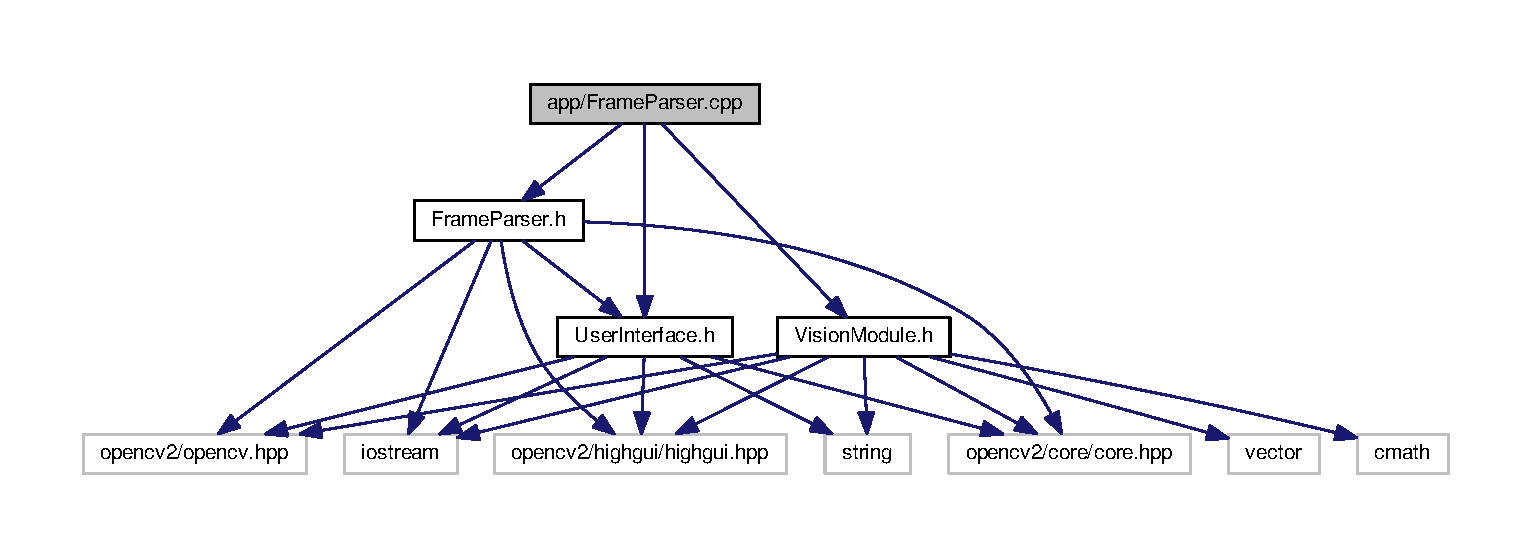
\includegraphics[width=350pt]{FrameParser_8cpp__incl}
\end{center}
\end{figure}


\subsection{Detailed Description}
Implements \hyperlink{classFrameParser}{Frame\+Parser} class methods. 

\begin{DoxyAuthor}{Author}
Saimouli Katragadda (saimouli) 

Adarsh Jagan Sathyamoorthy 
\end{DoxyAuthor}
\begin{DoxyCopyright}{Copyright}
M\+IT License 
\end{DoxyCopyright}

\hypertarget{VisionModule_8cpp}{}\section{app/\+Vision\+Module.cpp File Reference}
\label{VisionModule_8cpp}\index{app/\+Vision\+Module.\+cpp@{app/\+Vision\+Module.\+cpp}}


Implements \hyperlink{classVisionModule}{Vision\+Module} class methods.  


{\ttfamily \#include \char`\"{}Vision\+Module.\+h\char`\"{}}\\*
Include dependency graph for Vision\+Module.\+cpp\+:
\nopagebreak
\begin{figure}[H]
\begin{center}
\leavevmode
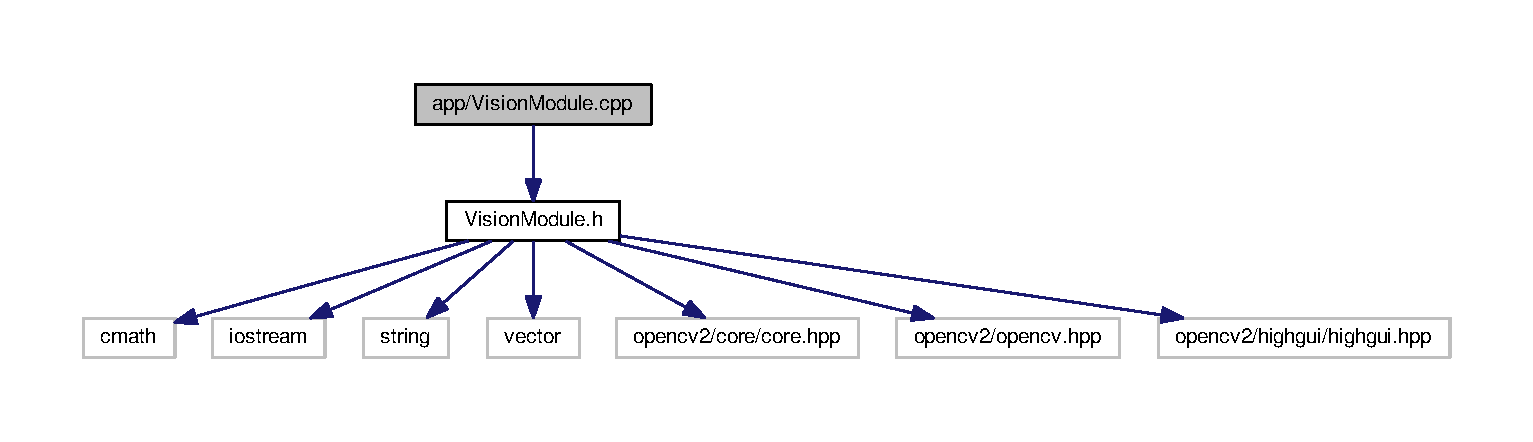
\includegraphics[width=350pt]{VisionModule_8cpp__incl}
\end{center}
\end{figure}


\subsection{Detailed Description}
Implements \hyperlink{classVisionModule}{Vision\+Module} class methods. 

\begin{DoxyAuthor}{Author}
Saimouli Katragadda (saimouli) 
\end{DoxyAuthor}
\begin{DoxyCopyright}{Copyright}
M\+IT License 
\end{DoxyCopyright}

\hypertarget{FrameParser_8h}{}\section{include/\+Frame\+Parser.h File Reference}
\label{FrameParser_8h}\index{include/\+Frame\+Parser.\+h@{include/\+Frame\+Parser.\+h}}


\hyperlink{classFrameParser}{Frame\+Parser} Class declaration  Declared functions Class to extract frames from the video input, and process frames.  


{\ttfamily \#include $<$iostream$>$}\\*
{\ttfamily \#include $<$opencv2/core/core.\+hpp$>$}\\*
{\ttfamily \#include $<$opencv2/opencv.\+hpp$>$}\\*
{\ttfamily \#include $<$opencv2/highgui/highgui.\+hpp$>$}\\*
{\ttfamily \#include \char`\"{}User\+Interface.\+h\char`\"{}}\\*
Include dependency graph for Frame\+Parser.\+h\+:
\nopagebreak
\begin{figure}[H]
\begin{center}
\leavevmode
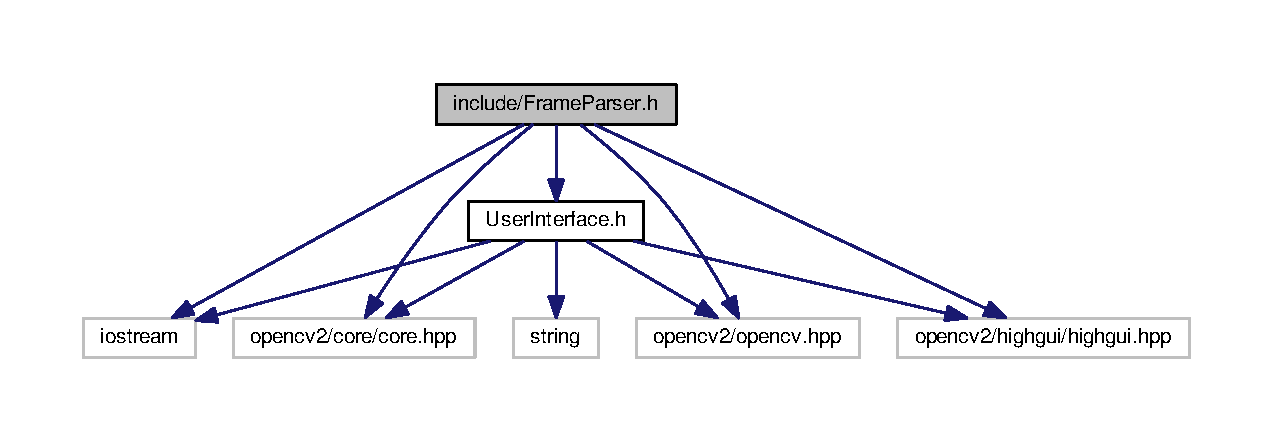
\includegraphics[width=350pt]{FrameParser_8h__incl}
\end{center}
\end{figure}
This graph shows which files directly or indirectly include this file\+:
\nopagebreak
\begin{figure}[H]
\begin{center}
\leavevmode
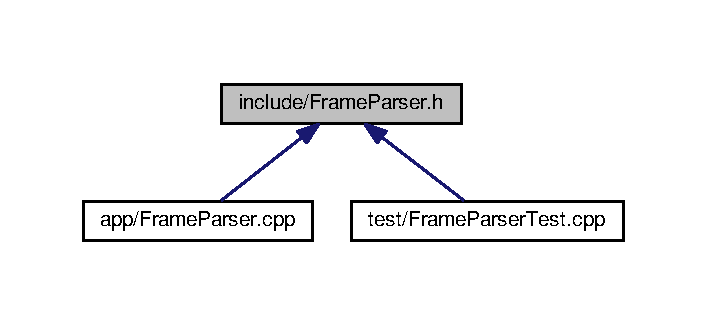
\includegraphics[width=340pt]{FrameParser_8h__dep__incl}
\end{center}
\end{figure}
\subsection*{Classes}
\begin{DoxyCompactItemize}
\item 
class \hyperlink{classFrameParser}{Frame\+Parser}
\begin{DoxyCompactList}\small\item\em Class \hyperlink{classFrameParser}{Frame\+Parser} The following class \hyperlink{classFrameParser}{Frame\+Parser} aids \hyperlink{classUserInterface}{User\+Interface} class by parsing the frames in a video and calling the \hyperlink{classVisionModule}{Vision\+Module} and \hyperlink{classUserInterface}{User\+Interface} class for further image processing using Open\+CV. \end{DoxyCompactList}\end{DoxyCompactItemize}


\subsection{Detailed Description}
\hyperlink{classFrameParser}{Frame\+Parser} Class declaration  Declared functions Class to extract frames from the video input, and process frames. 

\begin{DoxyAuthor}{Author}
Saimouli Katragadda (saimouli) 

Adarsh Jagan Sathyamoorthy 
\end{DoxyAuthor}
\begin{DoxyCopyright}{Copyright}
M\+IT License 
\end{DoxyCopyright}

\hypertarget{UserInterface_8h}{}\section{include/\+User\+Interface.h File Reference}
\label{UserInterface_8h}\index{include/\+User\+Interface.\+h@{include/\+User\+Interface.\+h}}


\hyperlink{classUserInterface}{User\+Interface} Class declaration  Declared function Class to interact with user about the input format and to display the lanes and text on top of the video.  


{\ttfamily \#include $<$iostream$>$}\\*
{\ttfamily \#include $<$string$>$}\\*
{\ttfamily \#include $<$opencv2/core/core.\+hpp$>$}\\*
{\ttfamily \#include $<$opencv2/opencv.\+hpp$>$}\\*
{\ttfamily \#include $<$opencv2/highgui/highgui.\+hpp$>$}\\*
Include dependency graph for User\+Interface.\+h\+:
\nopagebreak
\begin{figure}[H]
\begin{center}
\leavevmode
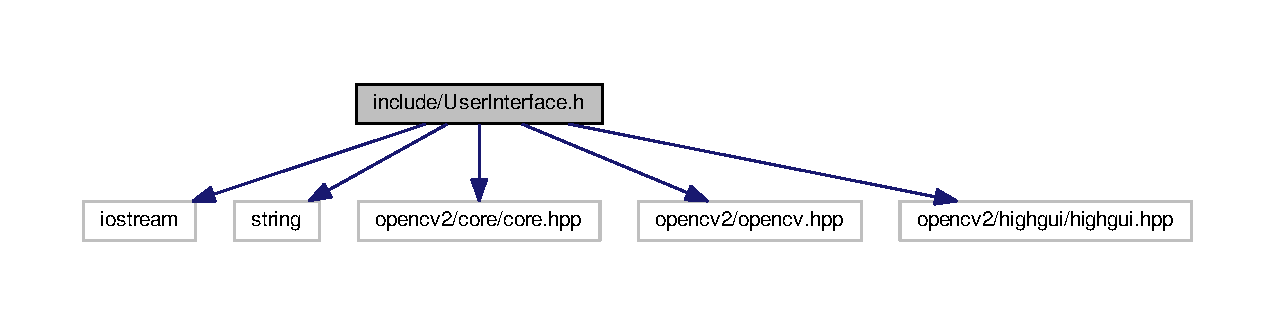
\includegraphics[width=350pt]{UserInterface_8h__incl}
\end{center}
\end{figure}
This graph shows which files directly or indirectly include this file\+:
\nopagebreak
\begin{figure}[H]
\begin{center}
\leavevmode
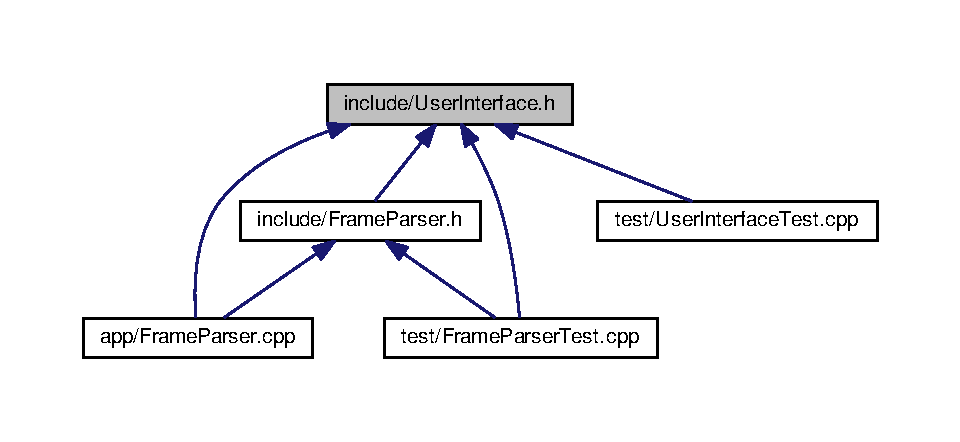
\includegraphics[width=350pt]{UserInterface_8h__dep__incl}
\end{center}
\end{figure}
\subsection*{Classes}
\begin{DoxyCompactItemize}
\item 
class \hyperlink{classUserInterface}{User\+Interface}
\begin{DoxyCompactList}\small\item\em Class \hyperlink{classUserInterface}{User\+Interface} The following class \hyperlink{classUserInterface}{User\+Interface} gets the user input and interacts with the \hyperlink{classVisionModule}{Vision\+Module} class. It augments the output from \hyperlink{classVisionModule}{Vision\+Module} class onto the user input. \end{DoxyCompactList}\end{DoxyCompactItemize}


\subsection{Detailed Description}
\hyperlink{classUserInterface}{User\+Interface} Class declaration  Declared function Class to interact with user about the input format and to display the lanes and text on top of the video. 

\begin{DoxyAuthor}{Author}
Saimouli Katragadda (saimouli) 

Adarsh Jagan Sathyamoorthy 
\end{DoxyAuthor}
\begin{DoxyCopyright}{Copyright}
M\+IT License 
\end{DoxyCopyright}

\hypertarget{VisionModule_8h}{}\section{include/\+Vision\+Module.h File Reference}
\label{VisionModule_8h}\index{include/\+Vision\+Module.\+h@{include/\+Vision\+Module.\+h}}


\hyperlink{classVisionModule}{Vision\+Module} Class declaration  Declared functions Class to denoise frames, apply homography, apply histogram, and find heading angle.  


{\ttfamily \#include $<$cmath$>$}\\*
{\ttfamily \#include $<$iostream$>$}\\*
{\ttfamily \#include $<$string$>$}\\*
{\ttfamily \#include $<$vector$>$}\\*
{\ttfamily \#include $<$opencv2/core/core.\+hpp$>$}\\*
{\ttfamily \#include $<$opencv2/opencv.\+hpp$>$}\\*
{\ttfamily \#include $<$opencv2/highgui/highgui.\+hpp$>$}\\*
Include dependency graph for Vision\+Module.\+h\+:
\nopagebreak
\begin{figure}[H]
\begin{center}
\leavevmode
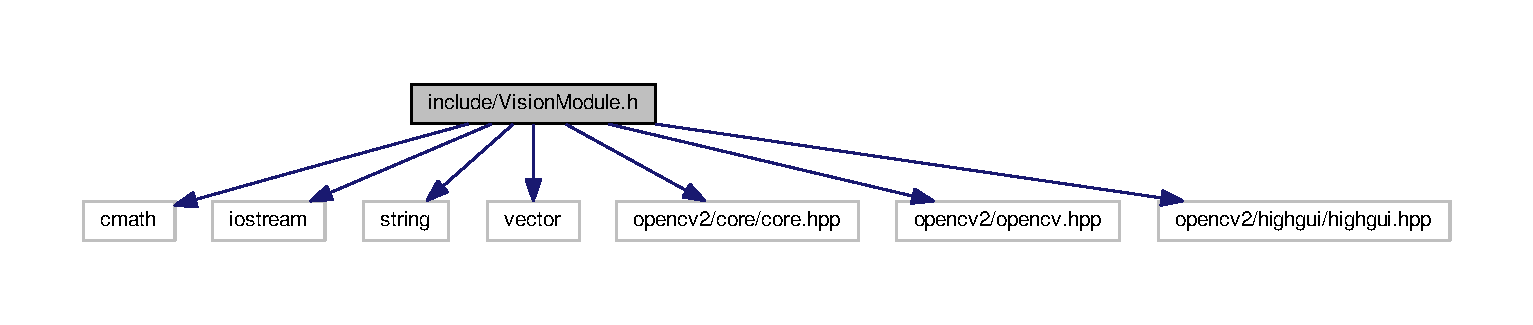
\includegraphics[width=350pt]{VisionModule_8h__incl}
\end{center}
\end{figure}
This graph shows which files directly or indirectly include this file\+:
\nopagebreak
\begin{figure}[H]
\begin{center}
\leavevmode
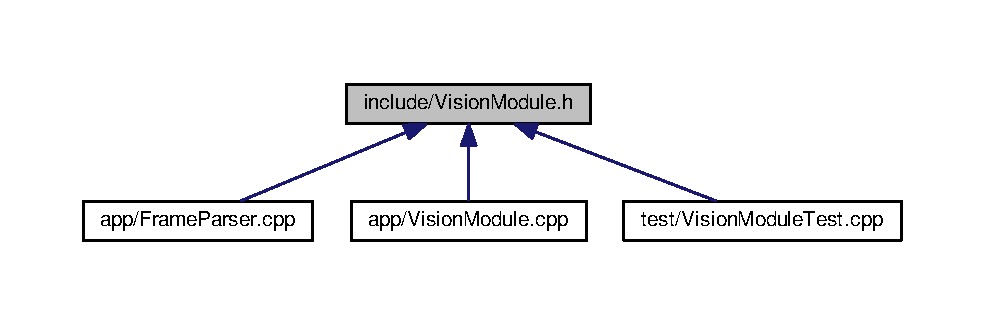
\includegraphics[width=350pt]{VisionModule_8h__dep__incl}
\end{center}
\end{figure}
\subsection*{Classes}
\begin{DoxyCompactItemize}
\item 
class \hyperlink{classVisionModule}{Vision\+Module}
\begin{DoxyCompactList}\small\item\em Class \hyperlink{classVisionModule}{Vision\+Module} The following class \hyperlink{classVisionModule}{Vision\+Module} gets the frames from \hyperlink{classFrameParser}{Frame\+Parser} class and is responsible for filtering and detecting hough lines on to an image. \end{DoxyCompactList}\end{DoxyCompactItemize}


\subsection{Detailed Description}
\hyperlink{classVisionModule}{Vision\+Module} Class declaration  Declared functions Class to denoise frames, apply homography, apply histogram, and find heading angle. 

\begin{DoxyAuthor}{Author}
Saimouli Katragadda (saimouli) 

Adarsh Jagan Sathyamoorthy 
\end{DoxyAuthor}
\begin{DoxyCopyright}{Copyright}
M\+IT License 
\end{DoxyCopyright}

\hypertarget{FrameParserTest_8cpp}{}\section{test/\+Frame\+Parser\+Test.cpp File Reference}
\label{FrameParserTest_8cpp}\index{test/\+Frame\+Parser\+Test.\+cpp@{test/\+Frame\+Parser\+Test.\+cpp}}


Implements tests for \hyperlink{classFrameParser}{Frame\+Parser} class methods.  


{\ttfamily \#include $<$gtest/gtest.\+h$>$}\\*
{\ttfamily \#include $<$gmock/gmock.\+h$>$}\\*
{\ttfamily \#include $<$vector$>$}\\*
{\ttfamily \#include \char`\"{}Frame\+Parser.\+h\char`\"{}}\\*
{\ttfamily \#include \char`\"{}User\+Interface.\+h\char`\"{}}\\*
{\ttfamily \#include $<$cmath$>$}\\*
{\ttfamily \#include $<$iostream$>$}\\*
Include dependency graph for Frame\+Parser\+Test.\+cpp\+:
\nopagebreak
\begin{figure}[H]
\begin{center}
\leavevmode
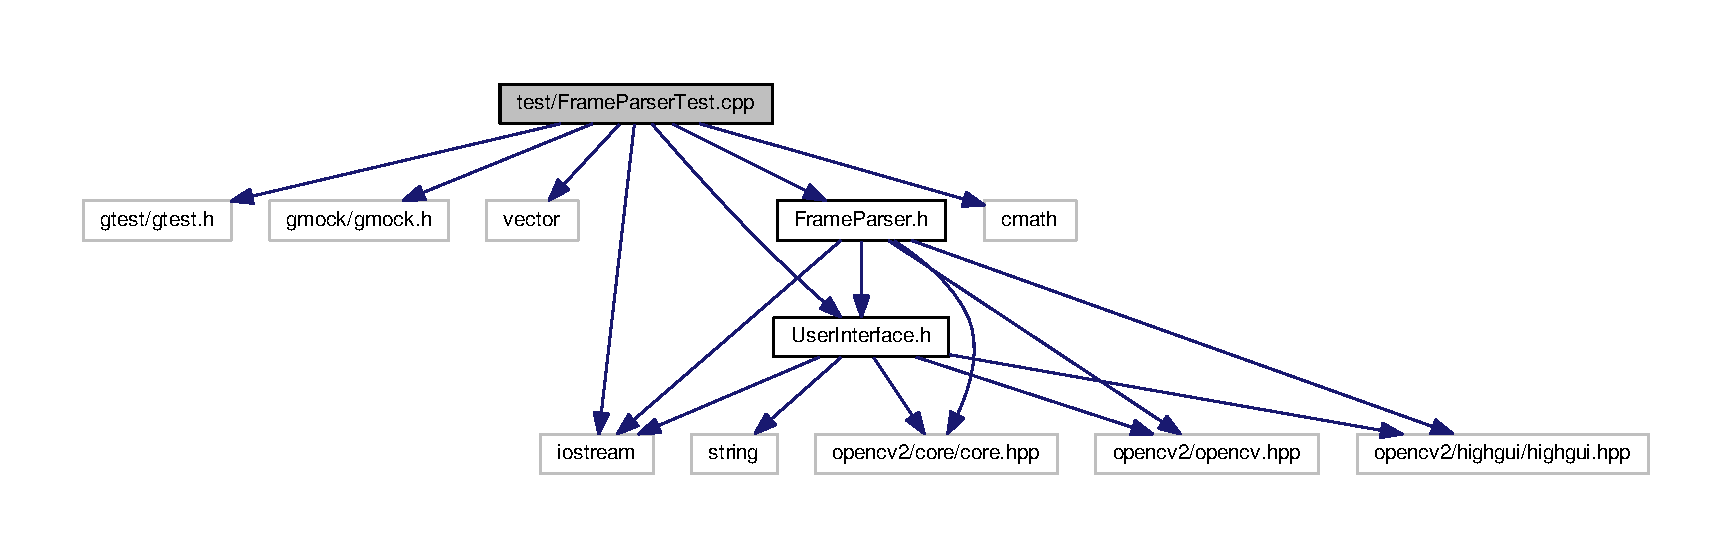
\includegraphics[width=350pt]{FrameParserTest_8cpp__incl}
\end{center}
\end{figure}
\subsection*{Functions}
\begin{DoxyCompactItemize}
\item 
\hyperlink{FrameParserTest_8cpp_ab133880284a41aab0429dd0fdcf56de8}{T\+E\+ST} (extract\+Frames\+Check, test\+Proper\+Returns\+After\+Good\+Run)
\begin{DoxyCompactList}\small\item\em Case to test if extract\+Frame functions executes successfully. \end{DoxyCompactList}\end{DoxyCompactItemize}


\subsection{Detailed Description}
Implements tests for \hyperlink{classFrameParser}{Frame\+Parser} class methods. 

\begin{DoxyAuthor}{Author}
Saimouli Katragadda (saimouli) 

Adarsh Jagan Sathyamoorthy 
\end{DoxyAuthor}
\begin{DoxyCopyright}{Copyright}
M\+IT License Copyright (c) 2018 Saimouli Katragadda, Adarsh Jagan Sathyamoorthy 
\end{DoxyCopyright}


\subsection{Function Documentation}
\index{Frame\+Parser\+Test.\+cpp@{Frame\+Parser\+Test.\+cpp}!T\+E\+ST@{T\+E\+ST}}
\index{T\+E\+ST@{T\+E\+ST}!Frame\+Parser\+Test.\+cpp@{Frame\+Parser\+Test.\+cpp}}
\subsubsection[{\texorpdfstring{T\+E\+S\+T(extract\+Frames\+Check, test\+Proper\+Returns\+After\+Good\+Run)}{TEST(extractFramesCheck, testProperReturnsAfterGoodRun)}}]{\setlength{\rightskip}{0pt plus 5cm}T\+E\+ST (
\begin{DoxyParamCaption}
\item[{extract\+Frames\+Check}]{, }
\item[{test\+Proper\+Returns\+After\+Good\+Run}]{}
\end{DoxyParamCaption}
)}\hypertarget{FrameParserTest_8cpp_ab133880284a41aab0429dd0fdcf56de8}{}\label{FrameParserTest_8cpp_ab133880284a41aab0429dd0fdcf56de8}


Case to test if extract\+Frame functions executes successfully. 


\begin{DoxyParams}{Parameters}
{\em none} & \\
\hline
\end{DoxyParams}
\begin{DoxyReturn}{Returns}
none 
\end{DoxyReturn}

\hypertarget{UserInterfaceTest_8cpp}{}\section{test/\+User\+Interface\+Test.cpp File Reference}
\label{UserInterfaceTest_8cpp}\index{test/\+User\+Interface\+Test.\+cpp@{test/\+User\+Interface\+Test.\+cpp}}


Unit test for the \hyperlink{classUserInterface}{User\+Interface} class.  


{\ttfamily \#include $<$gtest/gtest.\+h$>$}\\*
{\ttfamily \#include $<$iostream$>$}\\*
{\ttfamily \#include \char`\"{}User\+Interface.\+h\char`\"{}}\\*
Include dependency graph for User\+Interface\+Test.\+cpp\+:
\nopagebreak
\begin{figure}[H]
\begin{center}
\leavevmode
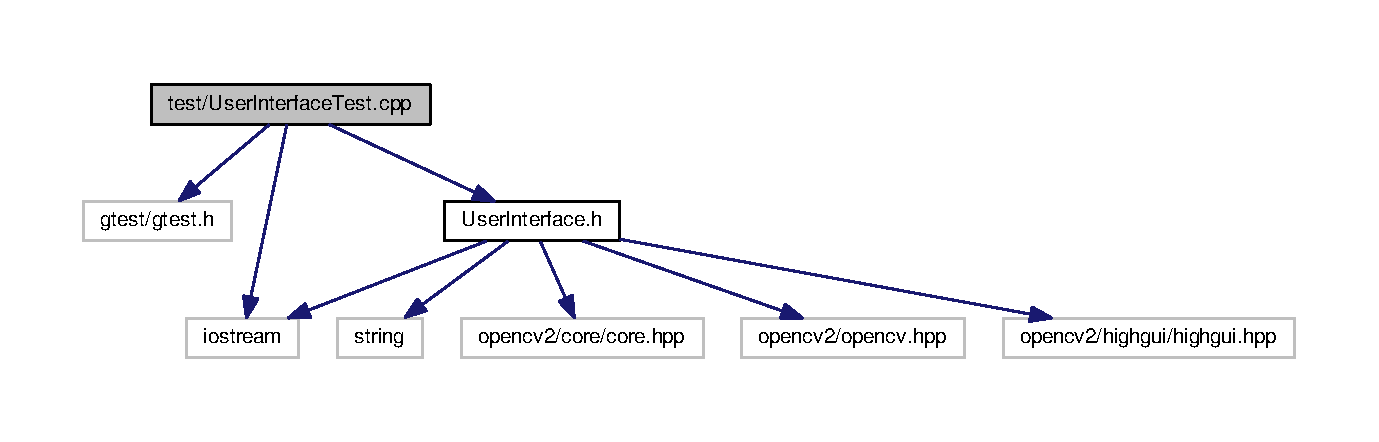
\includegraphics[width=350pt]{UserInterfaceTest_8cpp__incl}
\end{center}
\end{figure}
\subsection*{Functions}
\begin{DoxyCompactItemize}
\item 
\hyperlink{UserInterfaceTest_8cpp_ac87eebd65fb78cdb586c3ed1d2827803}{T\+E\+ST} (User\+Interfacetest, User\+Choice\+Method\+Test)
\begin{DoxyCompactList}\small\item\em case to test user initialization \end{DoxyCompactList}\end{DoxyCompactItemize}


\subsection{Detailed Description}
Unit test for the \hyperlink{classUserInterface}{User\+Interface} class. 

\begin{DoxyAuthor}{Author}
Saimouli Katragadda (saimouli) 

Adarsh Jagan Sathyamoorthy 
\end{DoxyAuthor}
\begin{DoxyCopyright}{Copyright}
M\+IT License Copyright (c) 2018 Saimouli Katragadda, Adarsh Jagan Sathyamoorthy 
\end{DoxyCopyright}


\subsection{Function Documentation}
\index{User\+Interface\+Test.\+cpp@{User\+Interface\+Test.\+cpp}!T\+E\+ST@{T\+E\+ST}}
\index{T\+E\+ST@{T\+E\+ST}!User\+Interface\+Test.\+cpp@{User\+Interface\+Test.\+cpp}}
\subsubsection[{\texorpdfstring{T\+E\+S\+T(\+User\+Interfacetest, User\+Choice\+Method\+Test)}{TEST(UserInterfacetest, UserChoiceMethodTest)}}]{\setlength{\rightskip}{0pt plus 5cm}T\+E\+ST (
\begin{DoxyParamCaption}
\item[{User\+Interfacetest}]{, }
\item[{User\+Choice\+Method\+Test}]{}
\end{DoxyParamCaption}
)}\hypertarget{UserInterfaceTest_8cpp_ac87eebd65fb78cdb586c3ed1d2827803}{}\label{UserInterfaceTest_8cpp_ac87eebd65fb78cdb586c3ed1d2827803}


case to test user initialization 


\begin{DoxyParams}{Parameters}
{\em none} & \\
\hline
\end{DoxyParams}
\begin{DoxyReturn}{Returns}
none 
\end{DoxyReturn}

\hypertarget{VisionModuleTest_8cpp}{}\section{test/\+Vision\+Module\+Test.cpp File Reference}
\label{VisionModuleTest_8cpp}\index{test/\+Vision\+Module\+Test.\+cpp@{test/\+Vision\+Module\+Test.\+cpp}}


Test for \hyperlink{classVisionModule}{Vision\+Module} class methods.  


{\ttfamily \#include $<$gtest/gtest.\+h$>$}\\*
{\ttfamily \#include $<$gmock/gmock.\+h$>$}\\*
{\ttfamily \#include $<$vector$>$}\\*
{\ttfamily \#include $<$Vision\+Module.\+h$>$}\\*
{\ttfamily \#include $<$cmath$>$}\\*
{\ttfamily \#include $<$iostream$>$}\\*
Include dependency graph for Vision\+Module\+Test.\+cpp\+:
\nopagebreak
\begin{figure}[H]
\begin{center}
\leavevmode
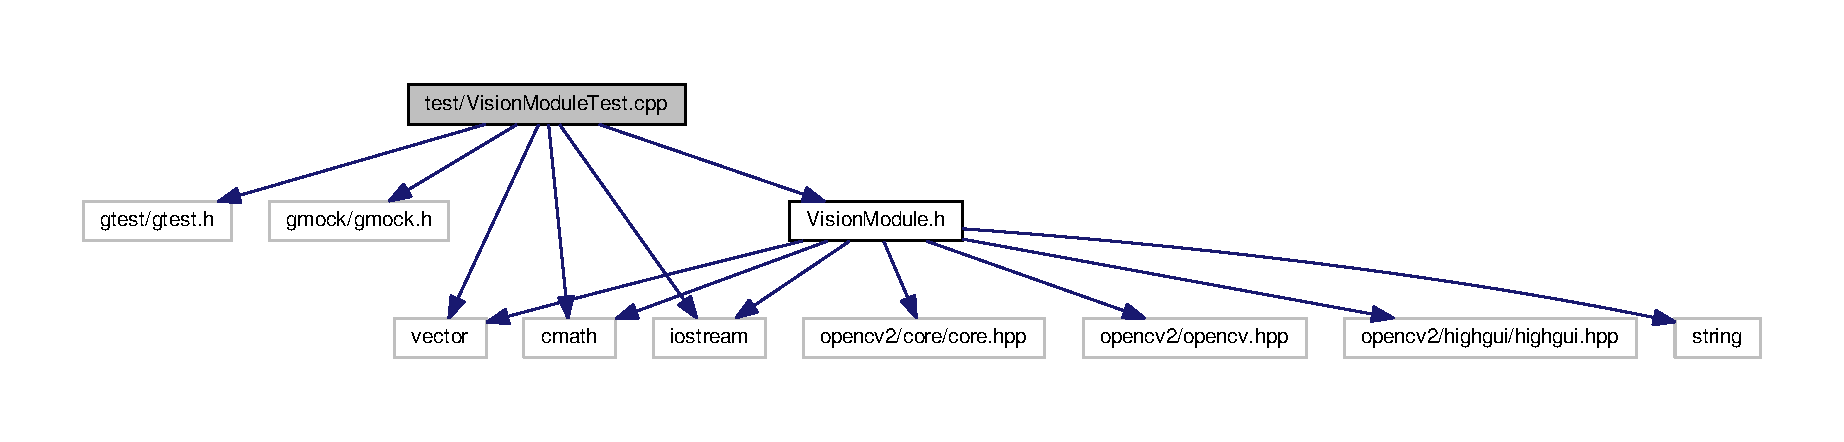
\includegraphics[width=350pt]{VisionModuleTest_8cpp__incl}
\end{center}
\end{figure}
\subsection*{Functions}
\begin{DoxyCompactItemize}
\item 
\hyperlink{VisionModuleTest_8cpp_aca4f0f061e5715dcadba05cbcde16425}{T\+E\+ST} (camera\+Matrix\+Check, testcamera\+Matrix\+Size)
\begin{DoxyCompactList}\small\item\em Case to test if Camera\+Matrix is 3x3 matrix. \end{DoxyCompactList}\item 
\hyperlink{VisionModuleTest_8cpp_aa92e5219c48d40f5a2301d457225b81c}{T\+E\+ST} (distortion\+Coeff\+Check, testdistortion\+Coeff\+Size)
\begin{DoxyCompactList}\small\item\em Case to test if distortion\+Coeff is a 5x1 matrix. \end{DoxyCompactList}\item 
\hyperlink{VisionModuleTest_8cpp_a10870cad788d7a27e6a1e5cfe1ba1b4e}{T\+E\+ST} (undistort\+Frame\+Check, test\+Undistorted\+Frame\+Size)
\begin{DoxyCompactList}\small\item\em Case to test if the frame size we get after resize is equal to the original image size. \end{DoxyCompactList}\item 
\hyperlink{VisionModuleTest_8cpp_a97c5fed7df3c2ef2f0c1b74447f4ad54}{T\+E\+ST} (smoothen\+Frame\+Check, test\+Non\+Aggressive\+Smoothing)
\begin{DoxyCompactList}\small\item\em Case to ensure that the image isn\textquotesingle{}t aggressively smoothened. \end{DoxyCompactList}\item 
\hyperlink{VisionModuleTest_8cpp_aef13c31355d152d8a00f5aa391a73eee}{T\+E\+ST} (pers\+Matrix\+Check, test\+Matrix\+Sizeand\+Inverse)
\begin{DoxyCompactList}\small\item\em Case to test the sizes of the calculated perspective transform matrices is 3x3 and the multiplication leads a matrix with non zero diagonal elements. \end{DoxyCompactList}\item 
\hyperlink{VisionModuleTest_8cpp_a0d379af9b7a0152379125f6967327ccf}{T\+E\+ST} (peak\+Value\+Check, test\+Left\+Right\+Histogram\+Peaks)
\begin{DoxyCompactList}\small\item\em Case to test if the returned peaks have the correct x coordinates. \end{DoxyCompactList}\item 
\hyperlink{VisionModuleTest_8cpp_ab7687a73dbba121fcb5c57757d3405b4}{T\+E\+ST} (centroid\+Heading\+Angle\+Check, check\+Centroid\+Vectorand\+Heading\+Angle)
\begin{DoxyCompactList}\small\item\em Case to test left and right centroid x coordinates for proper values and correct theta value. \end{DoxyCompactList}\end{DoxyCompactItemize}


\subsection{Detailed Description}
Test for \hyperlink{classVisionModule}{Vision\+Module} class methods. 

\begin{DoxyAuthor}{Author}
Saimouli Katragadda (saimouli) 

Adarsh Jagan Sathyamoorthy 
\end{DoxyAuthor}
\begin{DoxyCopyright}{Copyright}
M\+IT License Copyright (c) 2018 Saimouli Katragadda, Adarsh Jagan Sathyamoorthy 
\end{DoxyCopyright}


\subsection{Function Documentation}
\index{Vision\+Module\+Test.\+cpp@{Vision\+Module\+Test.\+cpp}!T\+E\+ST@{T\+E\+ST}}
\index{T\+E\+ST@{T\+E\+ST}!Vision\+Module\+Test.\+cpp@{Vision\+Module\+Test.\+cpp}}
\subsubsection[{\texorpdfstring{T\+E\+S\+T(camera\+Matrix\+Check, testcamera\+Matrix\+Size)}{TEST(cameraMatrixCheck, testcameraMatrixSize)}}]{\setlength{\rightskip}{0pt plus 5cm}T\+E\+ST (
\begin{DoxyParamCaption}
\item[{camera\+Matrix\+Check}]{, }
\item[{testcamera\+Matrix\+Size}]{}
\end{DoxyParamCaption}
)}\hypertarget{VisionModuleTest_8cpp_aca4f0f061e5715dcadba05cbcde16425}{}\label{VisionModuleTest_8cpp_aca4f0f061e5715dcadba05cbcde16425}


Case to test if Camera\+Matrix is 3x3 matrix. 


\begin{DoxyParams}{Parameters}
{\em none} & \\
\hline
\end{DoxyParams}
\begin{DoxyReturn}{Returns}
none 
\end{DoxyReturn}
\index{Vision\+Module\+Test.\+cpp@{Vision\+Module\+Test.\+cpp}!T\+E\+ST@{T\+E\+ST}}
\index{T\+E\+ST@{T\+E\+ST}!Vision\+Module\+Test.\+cpp@{Vision\+Module\+Test.\+cpp}}
\subsubsection[{\texorpdfstring{T\+E\+S\+T(distortion\+Coeff\+Check, testdistortion\+Coeff\+Size)}{TEST(distortionCoeffCheck, testdistortionCoeffSize)}}]{\setlength{\rightskip}{0pt plus 5cm}T\+E\+ST (
\begin{DoxyParamCaption}
\item[{distortion\+Coeff\+Check}]{, }
\item[{testdistortion\+Coeff\+Size}]{}
\end{DoxyParamCaption}
)}\hypertarget{VisionModuleTest_8cpp_aa92e5219c48d40f5a2301d457225b81c}{}\label{VisionModuleTest_8cpp_aa92e5219c48d40f5a2301d457225b81c}


Case to test if distortion\+Coeff is a 5x1 matrix. 


\begin{DoxyParams}{Parameters}
{\em none} & \\
\hline
\end{DoxyParams}
\begin{DoxyReturn}{Returns}
none 
\end{DoxyReturn}
\index{Vision\+Module\+Test.\+cpp@{Vision\+Module\+Test.\+cpp}!T\+E\+ST@{T\+E\+ST}}
\index{T\+E\+ST@{T\+E\+ST}!Vision\+Module\+Test.\+cpp@{Vision\+Module\+Test.\+cpp}}
\subsubsection[{\texorpdfstring{T\+E\+S\+T(undistort\+Frame\+Check, test\+Undistorted\+Frame\+Size)}{TEST(undistortFrameCheck, testUndistortedFrameSize)}}]{\setlength{\rightskip}{0pt plus 5cm}T\+E\+ST (
\begin{DoxyParamCaption}
\item[{undistort\+Frame\+Check}]{, }
\item[{test\+Undistorted\+Frame\+Size}]{}
\end{DoxyParamCaption}
)}\hypertarget{VisionModuleTest_8cpp_a10870cad788d7a27e6a1e5cfe1ba1b4e}{}\label{VisionModuleTest_8cpp_a10870cad788d7a27e6a1e5cfe1ba1b4e}


Case to test if the frame size we get after resize is equal to the original image size. 


\begin{DoxyParams}{Parameters}
{\em none} & \\
\hline
\end{DoxyParams}
\begin{DoxyReturn}{Returns}
none 
\end{DoxyReturn}
\index{Vision\+Module\+Test.\+cpp@{Vision\+Module\+Test.\+cpp}!T\+E\+ST@{T\+E\+ST}}
\index{T\+E\+ST@{T\+E\+ST}!Vision\+Module\+Test.\+cpp@{Vision\+Module\+Test.\+cpp}}
\subsubsection[{\texorpdfstring{T\+E\+S\+T(smoothen\+Frame\+Check, test\+Non\+Aggressive\+Smoothing)}{TEST(smoothenFrameCheck, testNonAggressiveSmoothing)}}]{\setlength{\rightskip}{0pt plus 5cm}T\+E\+ST (
\begin{DoxyParamCaption}
\item[{smoothen\+Frame\+Check}]{, }
\item[{test\+Non\+Aggressive\+Smoothing}]{}
\end{DoxyParamCaption}
)}\hypertarget{VisionModuleTest_8cpp_a97c5fed7df3c2ef2f0c1b74447f4ad54}{}\label{VisionModuleTest_8cpp_a97c5fed7df3c2ef2f0c1b74447f4ad54}


Case to ensure that the image isn\textquotesingle{}t aggressively smoothened. 


\begin{DoxyParams}{Parameters}
{\em none} & \\
\hline
\end{DoxyParams}
\begin{DoxyReturn}{Returns}
none 
\end{DoxyReturn}
\index{Vision\+Module\+Test.\+cpp@{Vision\+Module\+Test.\+cpp}!T\+E\+ST@{T\+E\+ST}}
\index{T\+E\+ST@{T\+E\+ST}!Vision\+Module\+Test.\+cpp@{Vision\+Module\+Test.\+cpp}}
\subsubsection[{\texorpdfstring{T\+E\+S\+T(pers\+Matrix\+Check, test\+Matrix\+Sizeand\+Inverse)}{TEST(persMatrixCheck, testMatrixSizeandInverse)}}]{\setlength{\rightskip}{0pt plus 5cm}T\+E\+ST (
\begin{DoxyParamCaption}
\item[{pers\+Matrix\+Check}]{, }
\item[{test\+Matrix\+Sizeand\+Inverse}]{}
\end{DoxyParamCaption}
)}\hypertarget{VisionModuleTest_8cpp_aef13c31355d152d8a00f5aa391a73eee}{}\label{VisionModuleTest_8cpp_aef13c31355d152d8a00f5aa391a73eee}


Case to test the sizes of the calculated perspective transform matrices is 3x3 and the multiplication leads a matrix with non zero diagonal elements. 


\begin{DoxyParams}{Parameters}
{\em none} & \\
\hline
\end{DoxyParams}
\begin{DoxyReturn}{Returns}
none 
\end{DoxyReturn}
\index{Vision\+Module\+Test.\+cpp@{Vision\+Module\+Test.\+cpp}!T\+E\+ST@{T\+E\+ST}}
\index{T\+E\+ST@{T\+E\+ST}!Vision\+Module\+Test.\+cpp@{Vision\+Module\+Test.\+cpp}}
\subsubsection[{\texorpdfstring{T\+E\+S\+T(peak\+Value\+Check, test\+Left\+Right\+Histogram\+Peaks)}{TEST(peakValueCheck, testLeftRightHistogramPeaks)}}]{\setlength{\rightskip}{0pt plus 5cm}T\+E\+ST (
\begin{DoxyParamCaption}
\item[{peak\+Value\+Check}]{, }
\item[{test\+Left\+Right\+Histogram\+Peaks}]{}
\end{DoxyParamCaption}
)}\hypertarget{VisionModuleTest_8cpp_a0d379af9b7a0152379125f6967327ccf}{}\label{VisionModuleTest_8cpp_a0d379af9b7a0152379125f6967327ccf}


Case to test if the returned peaks have the correct x coordinates. 


\begin{DoxyParams}{Parameters}
{\em none} & \\
\hline
\end{DoxyParams}
\begin{DoxyReturn}{Returns}
none 
\end{DoxyReturn}
\index{Vision\+Module\+Test.\+cpp@{Vision\+Module\+Test.\+cpp}!T\+E\+ST@{T\+E\+ST}}
\index{T\+E\+ST@{T\+E\+ST}!Vision\+Module\+Test.\+cpp@{Vision\+Module\+Test.\+cpp}}
\subsubsection[{\texorpdfstring{T\+E\+S\+T(centroid\+Heading\+Angle\+Check, check\+Centroid\+Vectorand\+Heading\+Angle)}{TEST(centroidHeadingAngleCheck, checkCentroidVectorandHeadingAngle)}}]{\setlength{\rightskip}{0pt plus 5cm}T\+E\+ST (
\begin{DoxyParamCaption}
\item[{centroid\+Heading\+Angle\+Check}]{, }
\item[{check\+Centroid\+Vectorand\+Heading\+Angle}]{}
\end{DoxyParamCaption}
)}\hypertarget{VisionModuleTest_8cpp_ab7687a73dbba121fcb5c57757d3405b4}{}\label{VisionModuleTest_8cpp_ab7687a73dbba121fcb5c57757d3405b4}


Case to test left and right centroid x coordinates for proper values and correct theta value. 


\begin{DoxyParams}{Parameters}
{\em none} & \\
\hline
\end{DoxyParams}
\begin{DoxyReturn}{Returns}
none 
\end{DoxyReturn}

%--- End generated contents ---

% Index
\backmatter
\newpage
\phantomsection
\clearemptydoublepage
\addcontentsline{toc}{chapter}{Index}
\printindex

\end{document}
